%% Chapter 6 : Forecasting Techniques in Brief

\section{Time Horizons for Solar Forecasting}
\
\
\
\
\textbf{Intra-Hour:} It is done for the period of 15 minutes to 2 hours. It is related to Ramping events, aand variability related to operations\\
\textbf{Intra-Day:} It is done for 1hour to 6 hours. It is related to Load following forecasting.\\
\textbf{Day-Ahead:} It is done for 1 Day to 3 days ahead. It is related to Unit commitment, transmission scheduling, and day ahead markets.\\

The Fig (\ref{figc5h1}) represents the time horizon concept with more clearity.

\begin{figure}[H]
\centering
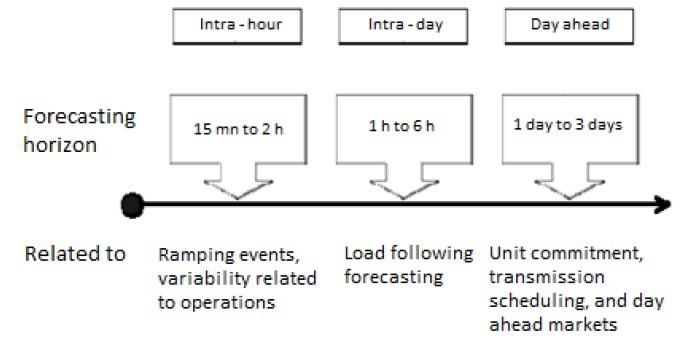
\includegraphics[scale=0.75]{ForecastIntro1}
\caption{Time Horizons for Solar Forecasting}
\label{figc5h1} %% to refer use, \ref{}
\end{figure}

\section{Solar Forecasting Models Classification}
\
\
\
\
Numerical Weather Forecasts: They are used for long time horizon forecasts. They predict weather by using present weather conditions as inputs to mathematical models. But, this model loses accuracy on a low spatial and temporal resolutions.\\

Classical Approaches: For long time horizons Time Series approach is utilized; forecast of solar energy is based on time series weather conditions and solar energy. For short time horizon cloud information is necessary. Here, models such as AR, MA, ARMA are used (these models are linear).\\

Artificial Neural Networks: They are used for short time horizon. These are non-linear models showing more flexibility in capturing the underlying characteristics of the data. Training of the model is involved over the known inputs and outputs. These models outperform short time classical approaches.\\

The Fig (\ref{figc5h2}) shows clearly the effectiveness of different forecasting models on the basis of time horizon and spatial resolution.


\begin{figure}[H]
\centering
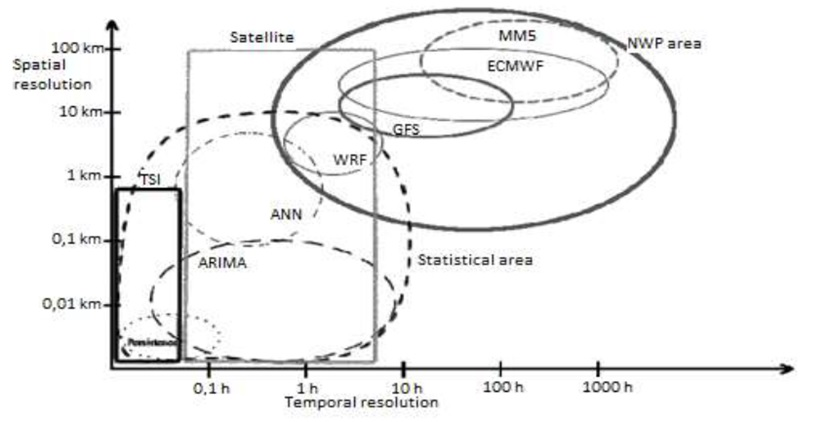
\includegraphics[scale=0.75]{ForecastIntro2}
\caption{Solar Forecasting Models (Spatial vs Temporal) Graph }
\label{figc5h1} %% to refer use, \ref{}
\end{figure}

\newpage

\subsubsection{Forecasting Using ARIMA Models}
\
\
\
\

\begin{figure}[H]
\centering
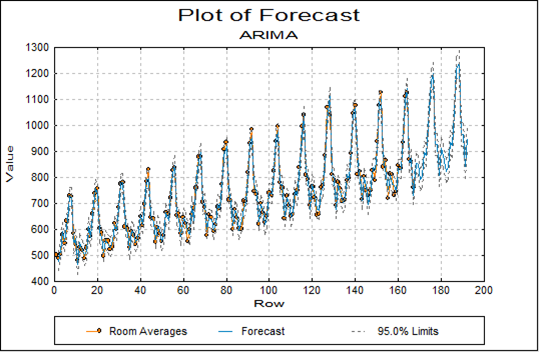
\includegraphics[scale=1]{Arima1}
\caption{A General ARIMA Model Forecast Graph}
\label{ari11} %% to refer use, \ref{}
\end{figure}

The first being the classical method of time series modeling propagated by the statisticians Box and Jenkins in the 70’s, and still used today. Their models of ARMA (Autoregressive Moving Averages, for stationary time series) and ARIMA (Autoregressive Integrated Moving Averages, for non-stationary time series) provide building blocks for creating the most basic statistical forecasts based on the time series’s mean and variance values.

\newpage

\subsubsection{Forecasting Using ANN }
\
\
\
\

\begin{figure}[H]
\centering
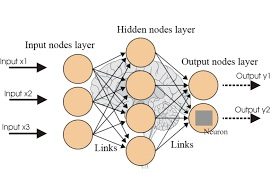
\includegraphics[scale=1]{ANN11}
\caption{Feed-Forward Neural Network Schematic}
\label{figc6h3} %% to refer use, \ref{}
\end{figure}

The second is the modern technique of Artificial Neural Networks, which are inspired from biological neural networks. They work on the principle of interconnected neurons forming a network between inputs and outputs; the neurons consists of a mathematical function, biases and weights. This network of neurons is made to learn the data during training phase using appropriate learning methods. ANN’s can be trained to do a variety of jobs; namely Clustering, Classification and Regression. For weather variable forecasting we need to develop a neural network for solving a regression problem. ANN’s are more effective than Time Series Models as they are not linear models, and are able to learn highly non-linear relationships between input and output; the only constraint being a good data set of training purposes.

\begin{figure}[H]
\centering
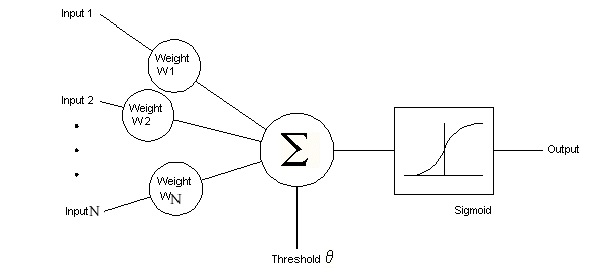
\includegraphics[scale=1]{ANN22}
\caption{Artificial Neuron Model}
\label{figc6h4} %% to refer use, \ref{}
\end{figure}

\newpage

\subsubsection{Forecasting Using WRF }
\
\
\
\
Finally we have the Numerical Weather Prediction Models (NWP’s) like ECMWF and WRF they produce good weather forecasts up to 1km spatial and about 3min temporal resolution. NWP’s are quite different from the first two forecasting techniques as they depend on accurate physical descriptions of the atmospheric processes and tend to give highly accurate forecasts. But, the problem here is these softwares require supercomputers to run them as they require a lot of computing power and memory.

\begin{figure}[H]
\centering
\includegraphics[scale=1]{wrf1}
\caption{WRF Software Schematic}
\label{figc6h5} %% to refer use, \ref{}
\end{figure}

